\documentclass[
  a4paper,
  oneside,
  BCOR = 10mm,
  DIV = 12,
  12pt,
  headings = normal,
]{scrartcl}

%%% Length calculations
\usepackage{calc}
%%%

%%% Support for color
\usepackage{xcolor}
\definecolor{lightblue}{HTML}{03A9F4}
\definecolor{red}{HTML}{F44336}
%%%

%%% Including graphics
\usepackage{graphicx}
%%%

%%% Font selection
\usepackage{fontspec}

\setromanfont{STIX Two Text}[
  SmallCapsFeatures = {LetterSpace = 8},
]

\setsansfont{IBM Plex Sans}[
  Scale = MatchUppercase,
]

\setmonofont{IBM Plex Mono}[
  Scale = MatchUppercase,
]
%%%

%%% Math typesetting
\usepackage{amsmath}

\usepackage{unicode-math}
\setmathfont{STIX Two Math}

\usepackage{IEEEtrantools}
%%%

%%% List settings
\usepackage{enumitem}
\setlist[enumerate]{
  label*      = {\arabic*.},
  left        = \parindent,
  topsep      = 0\baselineskip,
  parsep      = 0\baselineskip,
  noitemsep, % override itemsep
}
% List settings for levels 2–4
\setlist[enumerate, 2, 3, 4]{
  label*      = {\arabic*.},
  left        = 0em,
  topsep      = 0\baselineskip,
  parsep      = 0\baselineskip,
  noitemsep, % override itemsep
}

\setlist[itemize]{
  label*      = {—},
  left        = \parindent,
  topsep      = 0\baselineskip,
  parsep      = 0\baselineskip,
  itemsep     = 1\baselineskip,
  noitemsep, % override itemsep
}

\setlist[description]{
  font        = {\rmfamily\upshape\bfseries},
  topsep      = 1\baselineskip,
  parsep      = 0\baselineskip,
  itemsep     = 0\baselineskip,
}

%%%

%%% Structural elements typesetting
\setkomafont{pagenumber}{\rmfamily\upshape}
\setkomafont{disposition}{\rmfamily\bfseries}

% Sectioning
\RedeclareSectionCommand[
  beforeskip = -1\baselineskip,
  afterskip  = 1\baselineskip,
  font       = {\normalsize\bfseries\scshape},
]{section}

\RedeclareSectionCommand[
  beforeskip = -1\baselineskip,
  afterskip  = 1\baselineskip,
  font       = {\normalsize\bfseries\itshape},
]{subsection}

\RedeclareSectionCommand[
  beforeskip = -1\baselineskip,
  afterskip  = 1\baselineskip,
  font       = {\normalsize\bfseries},
]{subsubsection}

\RedeclareSectionCommand[
  beforeskip = -1\baselineskip,
  afterskip  = -0.5em,
  font       = {\normalsize\mdseries\scshape\addfontfeatures{Letters = {UppercaseSmallCaps}}},
]{paragraph}
%%%

%%% Typographic enhancements
\usepackage{microtype}
%%%

%%% Language-specific settings
\usepackage{polyglossia}
\setmainlanguage{ukrainian}
\setotherlanguages{english}
%%%

%%% Captions
\usepackage{caption}
\usepackage{subcaption}

%\DeclareCaptionLabelFormat{closing}{#2)}
%\captionsetup[subtable]{labelformat = closing}

%\captionsetup[subfigure]{labelformat = closing}

\captionsetup[table]{
  aboveskip = 0\baselineskip,
  belowskip = 0\baselineskip,
}

\captionsetup[figure]{
  aboveskip = 1\baselineskip,
  belowskip = 0\baselineskip,
}

\captionsetup[subfigure]{
  labelformat = simple,
  labelformat = brace,
  justification = RaggedRight,
  singlelinecheck = false,
}
%%%

%%% Hyphenated ragged typesetting
\usepackage{ragged2e}
%%%

%%% Table typesetting
\usepackage{booktabs}
\usepackage{longtable}

\usepackage{multirow}

\usepackage{array}
\newcolumntype{v}[1]{>{\RaggedRight\arraybackslash\hspace{0pt}}p{#1}}
\newcolumntype{b}[1]{>{\Centering\arraybackslash\hspace{0pt}}p{#1}}
\newcolumntype{n}[1]{>{\RaggedLeft\arraybackslash\hspace{0pt}}p{#1}}
%%%

%%% Drawing
\usepackage{tikz}
\usepackage{tikzscale}
\usetikzlibrary{datavisualization}
\usetikzlibrary{datavisualization.formats.functions}
\usetikzlibrary{positioning}
\usetikzlibrary{patterns}
\usetikzlibrary{intersections}
\usetikzlibrary{arrows.meta} % Stealth arrow tips
\usetikzlibrary{graphs}
\usetikzlibrary{graphdrawing}
\usegdlibrary{trees}
\usetikzlibrary{quotes}

\usepackage{pgfplots}
\usepgfplotslibrary{fillbetween}
%%%

%%% SI units typesetting
\usepackage{siunitx}
\sisetup{
  output-decimal-marker = {,},
  exponent-product      = {\cdot},
  inter-unit-product    = \ensuremath{{} \cdot {}},
  per-mode              = symbol,
}
%%%

% Code Highlighting
\usepackage{minted}
\setmintedinline{
  style = bw,
  breaklines,
}

\newminted[bashterm]{text}{%
  autogobble,%
  breaklines,%
  style=bw,%
}

\newminted[codegeneric]{text}{%
  autogobble,%
  style=bw,%
  breaklines,%
  fontsize=\small,%
}

\newmintinline{bash}{%
}

\newmintinline[minttext]{text}{%
  breaklines,%
  breakanywhere,%
}

%%% Framing code listings
\usepackage{tcolorbox}
\tcbuselibrary{breakable}
\tcbuselibrary{minted}
\tcbuselibrary{skins}

% Text file listing
\newtcblisting[
  auto counter,
  list inside,
  number within = section,
]{listingplaintext}[3][]{%
  minted language = text,
  minted style    = bw,
  minted options  = {
    autogobble,
    linenos,
    tabsize = 4,
    breaklines,
    breakanywhere,
    fontsize = \footnotesize,
  },
  empty,
  sharp corners,
  coltitle = black,
  borderline horizontal = {1pt}{0pt}{black},
  titlerule = {0.5pt},
  titlerule style = {
    black,
  },
  toptitle = 0.3em,
  bottomtitle = 0.3em,
  before skip      = \intextsep,
  after  skip      = \intextsep,
  title            = {Лістинг \thetcbcounter: #2},
  list entry       = {\protect\numberline{\thetcbcounter}#2},
  left = 0em,
  right = 0em,
  %
  listing only,
  breakable,
  %
  label = {#3},%
}

\newtcbinputlisting[
  use counter from = listingplaintext,
  list inside,
  number within = section
]{\inputplaintext}[4][]{%
  minted language = text,
  minted style    = bw,
  minted options  = {
    autogobble,
    linenos,
    tabsize = 4,
    breaklines,
    breakanywhere,
    fontsize = \footnotesize,
  },
  empty,
  sharp corners,
  coltitle = black,
  borderline horizontal = {1pt}{0pt}{black},
  titlerule = {0.5pt},
  titlerule style = {
    black,
  },
  toptitle = 0.3em,
  bottomtitle = 0.3em,
  before skip      = \intextsep,
  after  skip      = \intextsep,
  title            = {Лістинг \thetcbcounter: #3},
  list entry       = {\protect\numberline{\thetcbcounter}#3},
  left = 0em,
  right = 0em,
  %
  listing file={#2},
  listing only,
  breakable,
  %
  label = {#4}
}

\newtcblisting[
  use counter from = listingplaintext,
  list inside,
  number within = section,
]{listingpython}[3][]{%
  minted language = python,
  minted style    = bw,
  minted options  = {
    autogobble,
    linenos,
    tabsize = 4,
    breaklines,
    breakanywhere,
    fontsize = \footnotesize,
  },
  empty,
  sharp corners,
  coltitle = black,
  borderline horizontal = {1pt}{0pt}{black},
  titlerule = {0.5pt},
  titlerule style = {
    black,
  },
  toptitle = 0.3em,
  bottomtitle = 0.3em,
  before skip      = \intextsep,
  after  skip      = \intextsep,
  title            = {Лістинг \thetcbcounter: #2},
  list entry       = {\protect\numberline{\thetcbcounter}#2},
  left = 0em,
  right = 0em,
  %
  listing only,
  breakable,
  %
  label = {#3},
  %
  #1%
}

\newtcbinputlisting[
  use counter from = listingplaintext,
  list inside,
  number within = section
]{\inputpython}[4][]{%
  minted language = python,
  minted style    = bw,
  minted options  = {
    autogobble,
    linenos,
    tabsize = 4,
    breaklines,
    breakanywhere,
    fontsize = \footnotesize,
  },
  empty,
  sharp corners,
  coltitle = black,
  borderline horizontal = {1pt}{0pt}{black},
  titlerule = {0.5pt},
  titlerule style = {
    black,
  },
  toptitle = 0.3em,
  bottomtitle = 0.3em,
  before skip      = \intextsep,
  after  skip      = \intextsep,
  title            = {Лістинг \thetcbcounter: #3},
  list entry       = {\protect\numberline{\thetcbcounter}#3},
  left = 0em,
  right = 0em,
  %
  listing file={#2},
  listing only,
  breakable,
  %
  label = {#4}
}

% Linux command-line listing
\newtcblisting{linuxterm}%
{%
  % Syntax highlighing options
  listing only,%
  minted language = bash,%
  minted options={%
    autogobble,%
    linenos%
  },%
  % Presentation options
  empty,%
  %% Margins
  sharp corners,%
  toptitle = 0.0em,%
  bottomtitle = 0.0em,%
  left = 0em,%
  right = 0em,%
  before skip = \intextsep,%
  after skip = \intextsep,%
}

\newtcblisting{linuxtermout}%
{%
  % Syntax highlighing options
  listing only,%
  minted language = text,%
  minted options={%
    autogobble,%
    linenos%
  },%
  % Presentation options
  empty,%
  %% Margins
  sharp corners,%
  toptitle = 0.0em,%
  bottomtitle = 0.0em,%
  left = 0em,%
  right = 0em,%
  before skip = \intextsep,%
  after skip = \intextsep,%
}

% Dockerfile listings
\newtcblisting[
  use counter from = listingplaintext,
  list inside,
  number within = section,
]{listingdocker}[3][]{%
  minted language = dockerfile,
  minted style    = bw,
  minted options  = {
    autogobble,%
    linenos,
    tabsize = 4,
    breaklines,
    breakanywhere,
    fontsize = \footnotesize,
  },
  empty,
  sharp corners,
  coltitle = black,
  borderline horizontal = {1pt}{0pt}{black},
  titlerule = {0.5pt},
  titlerule style = {
    black,
  },
  toptitle = 0.3em,
  bottomtitle = 0.3em,
  before skip      = \intextsep,
  after  skip      = \intextsep,
  title            = {Лістинг \thetcbcounter: #2},
  list entry       = {\protect\numberline{\thetcbcounter}#2},
  left = 0em,
  right = 0em,
  %
  listing only,
  breakable,
  %
  label = {#3},%
}

% Docker Compose listings
\newtcblisting[
  use counter from = listingplaintext,
  list inside,
  number within = section,
]{listingdockercompose}[3][]{%
  minted language = yaml,
  minted style    = bw,
  minted options  = {
    autogobble,%
    linenos,
    tabsize = 4,
    breaklines,
    breakanywhere,
    fontsize = \footnotesize,
  },
  empty,
  sharp corners,
  coltitle = black,
  borderline horizontal = {1pt}{0pt}{black},
  titlerule = {0.5pt},
  titlerule style = {
    black,
  },
  toptitle = 0.3em,
  bottomtitle = 0.3em,
  before skip      = \intextsep,
  after  skip      = \intextsep,
  title            = {Лістинг \thetcbcounter: #2},
  list entry       = {\protect\numberline{\thetcbcounter}#2},
  left = 0em,
  right = 0em,
  %
  listing only,
  breakable,
  %
  label = {#3},%
}


% Customize minted line numbers
\renewcommand{\theFancyVerbLine}{\ttfamily\scriptsize\arabic{FancyVerbLine}}

%%%

%%% Typeset menus and keys
\usepackage{menukeys}[
  os=win,
]
%%%

%%% Links and hyperreferences
\usepackage{hyperref}
\hypersetup{
  bookmarksnumbered = true,
  colorlinks      = false,
  linkbordercolor = red,
  urlbordercolor  = lightblue,
  pdfborderstyle  = {/S/U/W 1.5},
}
%%%

%%% Length adjustment

% Set baselineskip, default is 14.5 pt
\linespread{1.068966} % ~15.5 pt
\setlength{\emergencystretch}{1em}
\setlength{\parindent}{1.5em}
\newlength{\gridunitwidth}
\setlength{\gridunitwidth}{\textwidth / 12}
%%%

%%% Custom commands
\newcommand{\allcaps}[1]{%
  {%
    \addfontfeatures{%
      Letters = UppercaseSmallCaps,
      LetterSpace = 8,%
    }%
    #1%
  }%
}
\newcommand{\filename}[1]{\texttt{#1}}
\newcommand{\progname}[1]{\texttt{#1}}
\newcommand{\commandname}[1]{\texttt{#1}}
\newcommand{\modulename}[1]{\texttt{#1}}
\newcommand{\transeng}[1]{{англ.}~\textit{\textenglish{#1}}}
%%%

%%% Custom math commands
\newcommand{\longvar}[1]{\mathit{#1}}
\newcommand{\vect}[1]{\mathbfit{#1}}
\newcommand{\matr}[1]{\mathbfit{#1}}

\newcommand{\logequiv}{\mathrel{\Longleftrightarrow}} % Logically equivalent

\DeclareMathOperator*{\minimize}{min} % minimize for linear programs
%%%

\begin{document}

\begin{titlepage}
    \begin{center}
      Міністерство освіти і~науки України\\
      Національний авіаційний університет\\
      Факультет кібербезпеки, комп'ютерної та~програмної інженерії\\
      Кафедра комп'ютеризованих систем управління

      \vspace{\fill}
        Лабораторна робота №~1.4\\
        з~дисципліни «Системи штучного інтелекту»\\
        на~тему «Методи пошуку в просторі станів»

      \vspace{\fill}

      \begin{flushright}
        Виконала:\\
        студентка \allcaps{ФККПІ}\\
        групи \allcaps{СП}-425\\
        Ульчич І.\,Г.\\
        Перевірила:\\
        Росінська Г.\,П.
      \end{flushright}

      Київ 2019
    \end{center}
  \end{titlepage}

  \section{Завдання роботи}
    Ознайомитись з методами пошуку розв'язків інтелектуальних задач у просторі станів. Вивчити блок-схеми алгоритмів для всіх методів пошуку.

  \section{Хід~роботи}
    Щоб~виконати лабораторну роботу, необхідно розв'язати задачу комівояжера для~графа, заданого за~варіантом~(рис.~\ref{fig:task-graph}), тобто знайти такий найкоротший шлях, який відвідає усі~точки графа і~повернеться у~початкову точку.

    \begin{figure}[!htbp]
      \centering
      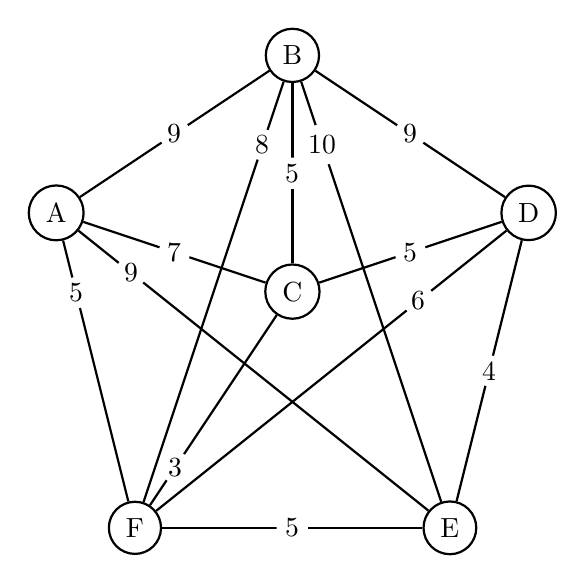
\begin{tikzpicture}
      \begin{scope}[every node/.style={circle,thick,draw}]
          \node (A) at (-3,2) {A};
          \node (B) at (0,4) {B};
          \node (C) at (0,1) {C};
          \node (D) at (3,2) {D};
          \node (E) at (2,-2) {E};
          \node (F) at (-2,-2) {F} ;
      \end{scope}

      \begin{scope}[
        >={Stealth},
        every node/.style={
          fill = white,
          circle,
          inner sep = 1pt,
        },
        every edge/.style={
          draw,
          thick
        }
      ]
          \path [-] (A) edge node[pos = 0.50] {$9$} (B);
          \path [-] (A) edge node[pos = 0.50] {$7$} (C);
          \path [-] (A) edge node[pos = 0.15] {$9$} (E);
          \path [-] (A) edge node[pos = 0.20] {$5$} (F);
          \path [-] (B) edge node[pos = 0.50] {$5$} (C);
          \path [-] (B) edge node[pos = 0.50] {$9$} (D);
          \path [-] (B) edge node[pos = 0.15] {$10$} (E);
          \path [-] (B) edge node[pos = 0.15] {$8$} (F);
          \path [-] (C) edge node[pos = 0.50] {$5$} (D);
          \path [-] (C) edge node[pos = 0.80] {$3$} (F);
          \path [-] (D) edge node[pos = 0.50] {$4$} (E);
          \path [-] (D) edge node[pos = 0.25] {$6$} (F);
          \path [-] (E) edge node[pos = 0.50] {$5$} (F);
      \end{scope}
      \end{tikzpicture}
      \caption{Граф, який описує умову задачі комівояжера}
      \label{fig:task-graph}
    \end{figure}

    Щоб~розв'язати задачу, розроблюємо програму, яка~шукатиме розв'язок задачі за~допомогою методу повного перебору можливих розв'язків у~просторі станів. Необхідно розв'язати задачу двома способами: перебор в ширину та в глибину. Розробивши програму~(лістинг~\ref{lst:source-code}), запускаємо її~і~спостерігаємо за~результатом~(рис.~\ref{fig:res-screenshot}). Як бачимо, програма знайшла такий найкоротший шлях:
    \[
      A \xrightarrow{9} B \xrightarrow{5} C \xrightarrow{5} D \xrightarrow{4} E \xrightarrow{5} F \xrightarrow{5} A = 33,
    \]
    перебравши можливі розв'язки у просторі станів двома обраними способами~(рис.~\ref{fig:graph-traversal-bfs}, \ref{fig:graph-traversal-dfs}).

    \begin{figure}[!htbp]
      \centering
      \begin{subfigure}[b]{6 \gridunitwidth - 1em / 2}
        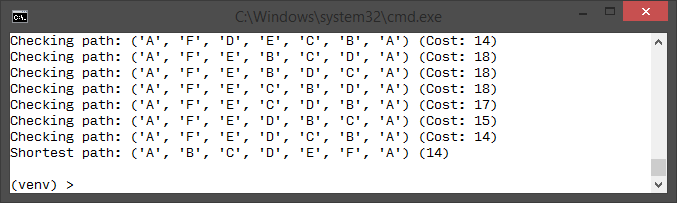
\includegraphics[width = \columnwidth]{./assets/00.png}
        \caption{Пошук вшир}
        \label{subfig:bfs}
      \end{subfigure}%
      \hspace{1em}%
      \begin{subfigure}[b]{6 \gridunitwidth - 1em / 2}
        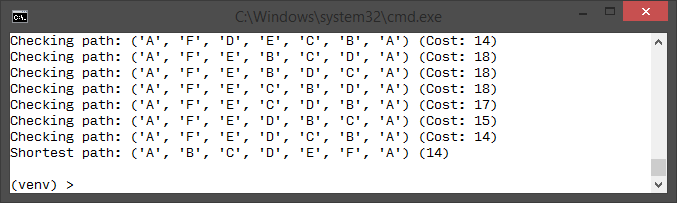
\includegraphics[width = \columnwidth]{./assets/01.png}
        \caption{Пошук вглиб}
        \label{subfig:dfs}
      \end{subfigure}
      \caption{Результат розв'язання задачі програмою}
      \label{fig:res-screenshot}
    \end{figure}

    \begin{figure}[!htbp]
      \centering
      \begin{tikzpicture}
        \begin{scope}[]
          \graph [
            trie, % A trie allows referencing a node multiple times in one path
            tree layout,
            math nodes,
            nodes = {
              rectangle,
              draw,
              thick,
            },
            edges = {
              > = Stealth,
              dashed,
            },
            typeset=\tikzgraphnodefullname,
          ] { [simple]
            A [label=left:1] -> {
              B [label=left:2] -> {
                C [label=left:3] -> {
                  D [label=left:7] -> {
                    E -> {
                      F -> {
                        A,
                      },
                    },
                    F -> "Z"[typeset={}, draw=none],
                    F -> "X"[typeset={}, draw=none],
                  },
                  E [label=left:8] -> "Z"[typeset={}, draw=none],
                  E -> "X"[typeset={}, draw=none],
                  F [label=right:9] -> "Z"[typeset={}, draw=none],
                  F -> "X"[typeset={}, draw=none],
                },
                D [label=left:4] -> "Z"[typeset={}, draw=none],
                D -> "X"[typeset={}, draw=none],
                E [label=left:5] -> "Z"[typeset={}, draw=none],
                E -> "X"[typeset={}, draw=none],
                F [label=left:6] -> "Z"[typeset={}, draw=none],
                F -> "X"[typeset={}, draw=none],
              },
            },
            {
              { [edges = {solid, thick}]
                A -> B -> C -> D -> E -> F -> A,
              }
            }
          };
        \end{scope}
      \end{tikzpicture}
      \caption{Частина графа пошуку розв'язку вшир}
      \label{fig:graph-traversal-bfs}
    \end{figure}

    \begin{figure}[!htbp]
      \centering
      \begin{tikzpicture}
        \begin{scope}[]
          \graph [
            trie, % A trie allows referencing a node multiple times in one path
            tree layout,
            math nodes,
            nodes = {
              rectangle,
              draw,
              thick,
            },
            edges = {
              > = Stealth,
              dashed,
            },
            typeset=\tikzgraphnodefullname,
          ] { [simple]
            A [label=left:1] -> {
              B [label=left:2] -> {
                C [label=left:3] -> {
                  D [label=left:4] -> {
                    E [label=left:5] -> {
                      F [label=left:6] -> {
                        A [label=left:7],
                      },
                    },
                    F [label=right:8] -> "Z"[typeset={}, draw=none],
                    F -> "X"[typeset={}, draw=none],
                  },
                  E -> "Z"[typeset={}, draw=none],
                  E -> "X"[typeset={}, draw=none],
                  F -> "Z"[typeset={}, draw=none],
                  F -> "X"[typeset={}, draw=none],
                },
                D -> "Z"[typeset={}, draw=none],
                D -> "X"[typeset={}, draw=none],
                E -> "Z"[typeset={}, draw=none],
                E -> "X"[typeset={}, draw=none],
                F -> "Z"[typeset={}, draw=none],
                F -> "X"[typeset={}, draw=none],
              },
            },
            {
              { [edges = {solid, thick}]
                A -> B -> C -> D -> E -> F -> A
              }
            }
          };
        \end{scope}
      \end{tikzpicture}
      \caption{Частина графа пошуку розв'язку вглиб}
      \label{fig:graph-traversal-dfs}
    \end{figure}

  \section{Висновок}
    Виконуючи дану лабораторну роботу, ми~дослідили процес породження простору станів і~ознайомились із~прикладами задач представлення у~просторі станів, а~також розробили програму для~розв'язання задачі комівояжера методом повного перебору розв'язків у~просторі станів.

  \appendix
  \section{Програма для~розв'язку поставленої задачі}

    \inputpython{../01-solution/solution.py}{Початковий код~програмного модуля для~розв'язання задачі комівояжера}{lst:source-code}

\end{document}
